\chapter[RESOLUCIÓN DE ECUACIONES BAJO RADICALES]{RESOLUCIÓN DE \\ ECUACIONES BAJO \\ RADICALES}\label{sec:radical}
\printchaptertableofcontents

\section{Introducción}

En el transcurso de la evolución histórica de las matemáticas, surge un punto de inflexión notable en el contexto del Renacimiento italiano con la publicación, en 1494, de \textit{Summa de Arithmetica} por Luca Pacioli. Este compendio exhaustivo, que abarcaba el panorama completo del conocimiento matemático de la época, dedicaba una sección especial a la enigmática ecuación cúbica. En aquel período, prevalecía la convicción de que dicha ecuación, representada por la forma
$$ax^3+bx^2+cx+d=0,$$
carecía de solución. Sin embargo, la ecuación cuadrática de la forma
$$ax^2 + bx + c = 0$$
había sido resuelta hace miles de años por muchas civilizaciones antiguas. Este paradigma desconcertante nos incita a una reflexión más profunda: ¿cómo es posible que una ecuación tan fundamental, aparentemente insuperable, desafiara a las mentes matemáticas más brillantes de aquel entonces? %Para abordar este enigma con lucidez, es imperativo sumergirse en las profundidades de la historia, a fin de comprender el desarrollo subyacente a esta conjetura enigmática.

\newpage

Por aquellos días, las matemáticas no se transcribían en ecuaciones, se escribían mediante palabras y dibujos. Por ejemplo, imaginemos que queremos resolver la ecuación
\begin{equation}
    x^2+26x=27. \label{ULTIMOYAYAYA}
\end{equation}
Los antiguos matemáticos pensaban al término $x^2$ como un cuadrado con lados que miden $x$; y $26x$ sería un rectángulo con un lado de largo igual a 26 y otro de largo $x$. Es decir:\marginElement{\justify
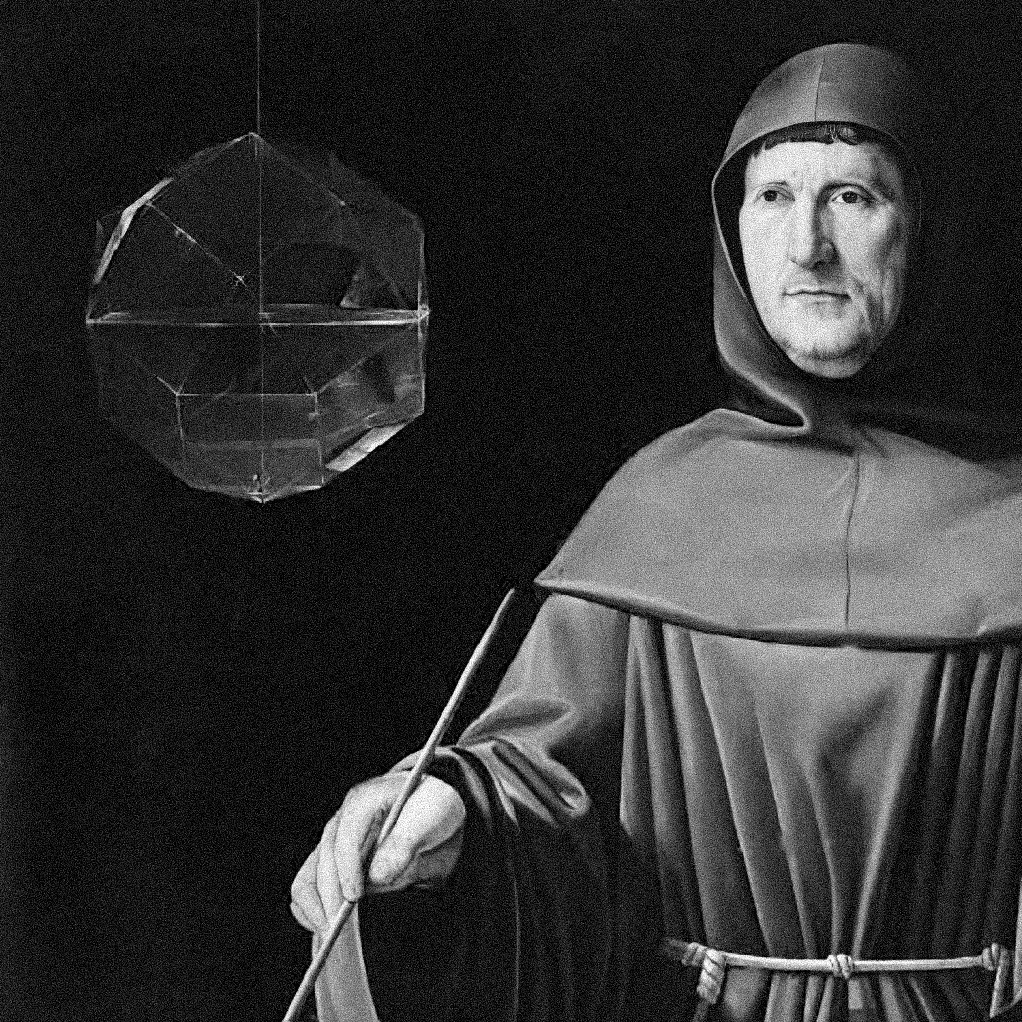
\includegraphics[width=\linewidth]{Images/ApendiceC/PACIOLI.jpeg}
\textbf{Luca Pacioli:} Nacido alrededor del 1446 en Borgo San Sepolcro, fue un matemático, franciscano y escritor italiano. Es considerado como el padre de la contabilidad moderna debido a su obra \textit{Summa de Arithmetica, Geometría, Proportioni et Proportionalità} en la que desarrolló el método de contabilidad de partida doble. Además de su trabajo en contabilidad, también hizo contribuciones significativas a la geometría y la teoría de la proporción en la que fue un hombre muy respetado, donde también trabajó como profesor y tutor en varias partes de Italia. Pacioli murió en 1517, pero su influencia en las matemáticas y la contabilidad ha sido duradera.
}
\begin{center}
    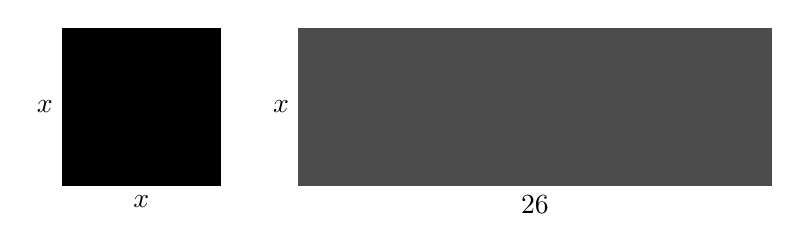
\begin{tikzpicture}
        \filldraw[black] (0,0) rectangle (2,2);
        \filldraw[black!70] (3,0) rectangle (9,2);
        
        \node at (0,1) [left] {$x$};
        \node at (1,0) [below] {$x$};
        
        \node at (6,0) [below] {$26$};
        \node at (3,1) [left] {$x$};
    \end{tikzpicture}
\end{center}
donde el área de las anteriores figuras suman 27.

Hagamos el siguiente arreglo:
\begin{center}
    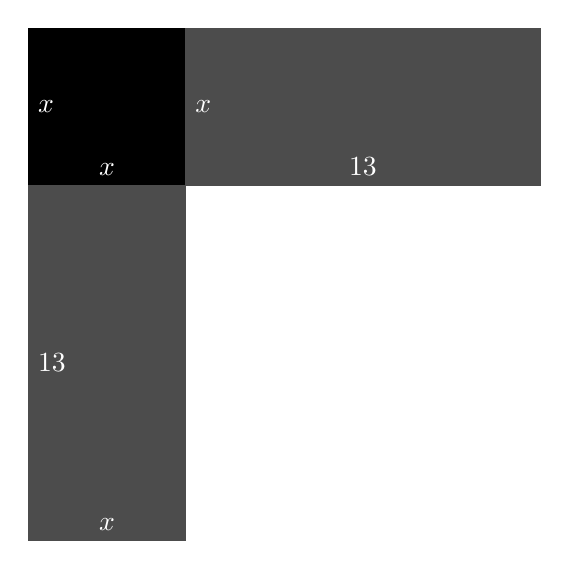
\begin{tikzpicture}
        \filldraw[black] (0,0) rectangle (2,2);
        
        \filldraw[black!70] (2,0) rectangle (6.5,2);
        
        \filldraw[black!70] (0,0) rectangle (2,-4.5);

        %\filldraw[black!80] (2,0) rectangle (6.5,-4.5);
        
        \node[white] at (0,1) [right] {$x$};
        \node[white] at (1,0) [above] {$x$};
        
        \node[white] at (2,1) [right] {$x$};
        \node[white] at (4.25,0) [above] {$13$};
        
        \node[white] at (0,-2.25) [right] {$13$};
        \node[white] at (1,-4.5) [above] {$x$};
    \end{tikzpicture}
\end{center}
pero podemos completar el cuadrado añadiendo un cuadrado de $13 \times 13$, es decir
\begin{center}
    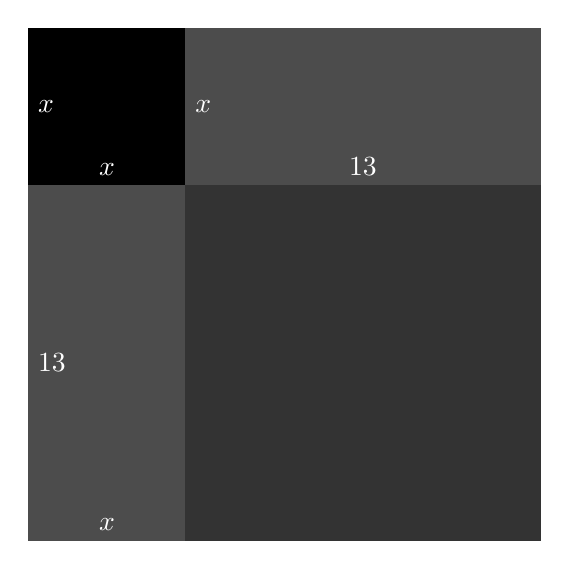
\begin{tikzpicture}
        \filldraw[black] (0,0) rectangle (2,2);
        
        \filldraw[black!70] (2,0) rectangle (6.5,2);
        
        \filldraw[black!70] (0,0) rectangle (2,-4.5);

        \filldraw[black!80] (2,0) rectangle (6.5,-4.5);
        
        \node[white] at (0,1) [right] {$x$};
        \node[white] at (1,0) [above] {$x$};
        
        \node[white] at (2,1) [right] {$x$};
        \node[white] at (4.25,0) [above] {$13$};
        
        \node[white] at (0,-2.25) [right] {$13$};
        \node[white] at (1,-4.5) [above] {$x$};
    \end{tikzpicture}
\end{center}
Ahora obtendríamos una nueva ecuación, la cual es
$$x^2+26x+169=196.$$

Sabiendo que la raíz cuadrada de $196$ es $14$, se tiene:
\marginElement{\justify
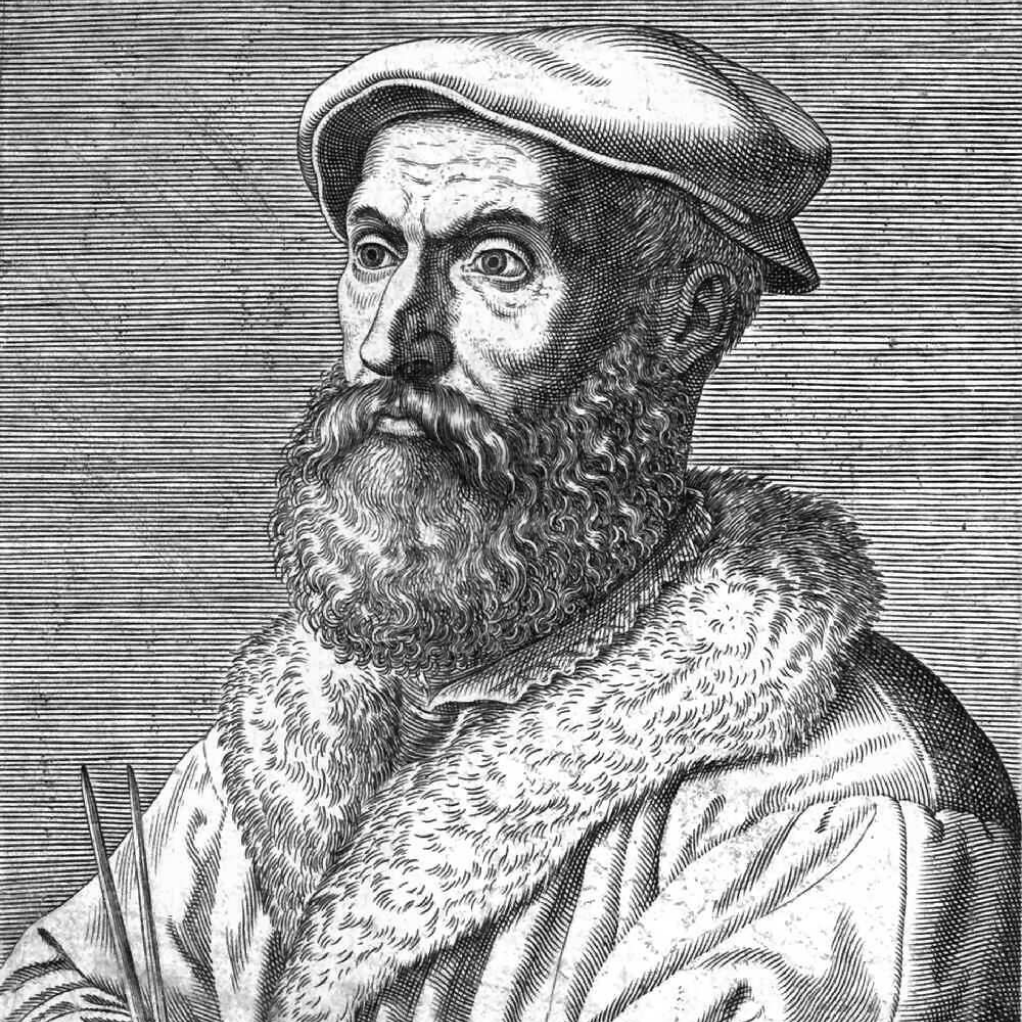
\includegraphics[width=\linewidth]{Images/ApendiceC/FONTANA.png}
\textbf{Niccolò Tartaglia:} Nacido en Brescia en 1499, es conocido por haber resuelto el problema de la cubatura, que consiste en determinar el volumen de una figura sólida. En 1543 publicó su obra \textit{Nova Scientia}, donde presentó sus descubrimientos en matemáticas y óptica, así como su método para resolver ecuaciones de tercer grado. Se le conocía por Tartaglia, ya que de niño había sufrido un corte en el rostro por parte de un soldado francés, lo que lo dejó tartamudo, de ahí se le conoce por \textit{tartaglia}, que es tartamudo en italiano. Tartaglia falleció en Venecia en 1557 y su legado ha sido reconocido por importantes matemáticos como Galileo Galilei y Johannes Kepler.
}
\begin{center}
    \begin{tikzpicture}
        \filldraw[black] (0,0) rectangle (2,2);
        
        \filldraw[black!70] (2,0) rectangle (6.5,2);
        
        \filldraw[black!70] (0,0) rectangle (2,-4.5);

        \filldraw[black!80] (2,0) rectangle (6.5,-4.5);
        
        \node[white] at (0,1) [right] {$x$};
        \node[white] at (1,0) [above] {$x$};
        
        \node[white] at (2,1) [right] {$x$};
        \node[white] at (4.25,0) [above] {$13$};
        
        \node[white] at (0,-2.25) [right] {$13$};
        \node[white] at (1,-4.5) [above] {$x$};

        \draw[snake=brace,thick] (6.6,2) -- (6.6,-4.5);
        
        \node at (6.7,-1.25) [right] {$14$};
    \end{tikzpicture}
\end{center}
Por lo que $x=1$. Lo anterior, es una forma visual de resolver una ecuación cuadrática, pero no es completa. Si $x=1$, podemos ver que es una solución de $x^2+26x=27$, pero también lo es $-27$. Por miles de años, los matemáticos ignoraban las soluciones negativas de sus ecuaciones porque  trataban con las cosas del mundo real (longitud, área y volumen). Para aquellos matemáticos, los números negativos no existían, se podía restar, pero no se podía tener una respuesta negativa ni coeficientes negativos. No existía una ecuación cuadrática como $ax^2+bx+c=0$, sino habían seis versiones diferentes para que los coeficientes siempre fueran positivos.

No fue hasta que Scipione Del Ferro, al rededor del año 1510, descubrió un método para resolver ecuaciones cúbicas reducidas, estas son una selección de ecuaciones cúbicas sin término elevado al cuadrado. Del Ferro no publicó sus resultados, ya que al mantener la solución en secreto, se aseguraba de mantener su empleo. Esto lo hizo durante casi dos décadas, y no fue hasta su lecho de muerte, en 1526, que se lo dejó entrever a su discípulo Antonio Maria del Fior. Luego de la muerte de Del Ferro, Fior desafío al gran matemático Niccolò Fontana Tartaglia, también italiano, a que resolviera un cierto número de ecuaciones de tercer grado. Fior no pudo resolver ni un solo problema, mientras que Tartaglia, antes del plazo fijado en este (40 días), encontró un método para resolver cualquier ecuación cúbica de la forma $x^3+px+q=0$. Antes del desafío, Tartaglia se entero que Fior se jactaba de haber resuelto la cúbica reducida, pero no lo creyó. Se corría el rumor de que un gran matemático le había revelado el secreto a Fior, lo que era más posible, así que sabiendo que una solución a la cúbica era posible y con su reputación en riesgo, se propuso resolver la cúbica reducida él mismo. Para hacerlo, exploró la idea de completar el cuadrado en tres dimensiones. Imaginemos que queremos resolver la ecuación
\begin{equation}
    x^3+9x=26 \label{ecuacioncardanoaresolver}
\end{equation}
entonces
\begin{multicols}{2}
    \begin{center}
        \begin{tikzpicture}[scale=0.8,
                    x  = {(0.5cm,0.5cm)},
                    y  = {(0.95cm,-0.25cm)},
                    z  = {(0cm,0.9cm)}]
            
            %%Cara izquierda%%
            \begin{scope}[canvas is yz plane at x=-1]
            
                \shade[left color=black!70,right color=black!80] (-1,-1) rectangle (1,1);
                \draw[black,decorate,decoration={brace,mirror,raise=4pt},thick,transform shape] (-1,-1) -- (1,-1);
                \draw[black,decorate,decoration={brace,raise=4pt},thick,transform shape] (-1,-1) -- (-1,1);
            \end{scope}
            
            \begin{scope}[canvas is xz plane at y=1]
            
                \shade[right color=black!60,left color=black!80] (-1,-1) rectangle (1,1);
                \draw[black,decorate,decoration={brace,mirror,raise=4pt},thick,transform shape] (-1,-1) -- (1,-1);
                \node[black] at (-5.9,3.2) [xscale=1] {$x$};
            \end{scope}
            
            \begin{scope}[canvas is yx plane at z=1]
            
                \shade[top color=black!90,bottom color=black!80] (-1,-1) rectangle (1,1);
                
                \node[black] at (3,-3.1) [xscale=1,transform shape,rotate=90] {\Large $x$};
                
                \node[black] at (1.6,-4.5) [xscale=1,transform shape] {\Large $x$};
                
                \node at (0,0) [xscale=1,transform shape,white] {$x^3$};
            \end{scope}
        \end{tikzpicture}
    \end{center}

\columnbreak

    \begin{flushleft}
        \begin{tikzpicture}[scale=0.8,
                    x  = {(0.5cm,0.5cm)},
                    y  = {(0.95cm,-0.25cm)},
                    z  = {(0cm,0.9cm)}]
            
            %%Segundo rectángulo%%
            \begin{scope}[canvas is yz plane at x=-1]
            
                \shade[left color=black!50,right color=black!70] (4,-1) rectangle (8,1);
            \end{scope}
            
            \begin{scope}[canvas is xz plane at y=5.368]
            
                \shade[right color=black!80,left color=black!70] (4,-4.509) rectangle (6,-2.509);
            \end{scope}
            
            \begin{scope}[canvas is yx plane at z=1]
            
                \shade[top color=black!90,bottom color=black!70] (4,-1) rectangle (8,1);
                
                \node at (6,0) [xscale=1,transform shape,white] {$9x$};
            \end{scope}
        \end{tikzpicture}
    \end{flushleft}
\end{multicols}
\noindent
donde la suma de los anteriores volúmenes sumen $26$.

Imaginemos extender tres lados del cubo $x^3$, una distancia $y$, es decir
\begin{center}
    \begin{tikzpicture}[scale=0.9,
                    x  = {(0.5cm,0.5cm)},
                    y  = {(0.95cm,-0.25cm)},
                    z  = {(0cm,0.9cm)}]

        \draw[dash pattern=on 3pt off 3pt] (-0.42,0.95) -- (-0.42,3) node [above] {$y$};
        %%Cara izquierda%%
        \begin{scope}[canvas is yz plane at x=-1]
            
            \shade[left color=black!70,right color=black!80] (-1,-1) rectangle (1,1);
        
        \end{scope}
            
        \begin{scope}[canvas is xz plane at y=1]

            \node[black] at (-5.6,3) [xscale=1] {$x$};
            
            \shade[right color=black!60,left color=black!80] (-1,-1) rectangle (1,1);

            \draw[dash pattern=on 3pt off 3pt] (-2.76,3) -- (-2.76,5) node [right] {$y$};
            
            \draw[dash pattern=on 3pt off 3pt] (-1.1,-1) -- (-2.8,-1) node [left] {$y$};
        \end{scope}
            
        \begin{scope}[canvas is yx plane at z=1]
            
            \shade[top color=black!90,bottom color=black!80] (-1,-1) rectangle (1,1);
                
            \node[black] at (3,-3.1) [xscale=1,transform shape,rotate=90] {\Large $x$};
                
            \node[black] at (1.6,-4.5) [xscale=1,transform shape] {\Large $x$};
                
            \node at (0,0) [xscale=1,transform shape,white] {$x^3$};
        \end{scope}
    \end{tikzpicture}
\end{center}
Por lo que se crea un nuevo cubo y más grande, cuyos lados ahora midan $z$, siendo $z=x+y$, es decir:
\begin{center}
    \begin{tikzpicture}[scale=1.1,
                    x  = {(0.5cm,0.5cm)},
                    y  = {(0.95cm,-0.25cm)},
                    z  = {(0cm,0.9cm)}]
        
        \begin{scope}[canvas is yz plane at x=-0.5]
        
            \shade[left color=black!50,right color=black!70] (-0.5,-0.5) rectangle (0.5,0.5);
        
        \end{scope}
        
        \begin{scope}[canvas is xz plane at y=0.5]
        
            \shade[right color=black!80,left color=black!70] (-0.5,-0.5) rectangle (0.5,0.5);
            
        \end{scope}
        
        \begin{scope}[canvas is yx plane at z=0.5]
        
            \shade[top color=black!90,bottom color=black!70] (-0.5,-0.5) rectangle (0.5,0.5);
            
        \end{scope}              
        
        %%Cara izquierda%%
        \begin{scope}[canvas is yz plane at x=-1]
        
            \shade[left color=black!20,right color=black!20,opacity=0.5] (-1,-1) rectangle (1,1);
            
            \draw[black,decorate,decoration={brace,mirror,raise=4pt},thick,transform shape] (-1,-1) -- (1,-1);
            \draw[black,decorate,decoration={brace,raise=4pt},thick,transform shape] (-1,-1) -- (-1,1);
            
        \end{scope}
        
        \begin{scope}[canvas is xz plane at y=1]
        
            \shade[right color=black!70,left color=black!20,opacity=0.5] (-1,-1) rectangle (1,1);
            \draw[black,decorate,decoration={brace,mirror,raise=4pt},thick,transform shape] (-1,-1) -- (1,-1);
            
            \node[black] at (-5.5,3.1) [xscale=1] {$z$};
            
        \end{scope}
        
        \begin{scope}[canvas is yx plane at z=1]
        
            \shade[top color=black!80,bottom color=black!20,opacity=0.5] (-1,-1) rectangle (1,1);
            
            \node[black] at (3,-3.1) [xscale=1,transform shape,rotate=90] {\footnotesize $z$};
            
            \node[black] at (1.6,-4.5) [xscale=1,transform shape] {\footnotesize $z$};
            
        \end{scope}
    \end{tikzpicture}
\end{center}
Podemos dividir el volumen adicional en siete formas:
\begin{center}
    \begin{tikzpicture}[scale=0.9,
                    x  = {(0.5cm,0.5cm)},
                    y  = {(0.95cm,-0.25cm)},
                    z  = {(0cm,0.9cm)}]
        %%%%CUBO CAFÉ%%%%
        %%Cara izquierda%%
        \begin{scope}[canvas is yz plane at x=-1]
            \shade[left color=black!50,right color=black!70] (-1,-4) rectangle (1,-2);
        \end{scope}
        
        %%Cara derecha%%
        \begin{scope}[canvas is xz plane at y=1]
            \shade[right color=black!80,left color=black!70] (-1,-4) rectangle (1,-2);
        \end{scope}
        
        %%Cara superior%%
        \begin{scope}[canvas is yx plane at z=-2]
            \shade[top color=black!90,bottom color=black!70] (-1,-1) rectangle (1,1);
        \end{scope}
        %%%%CUBO CAFÉ%%%%
        
        %%%%CUBO AZUL SUPERIOR%%%%
        %%Cara izquierda%%
        \begin{scope}[canvas is yz plane at x=-1]
            \shade[left color=black!50,right color=black!20] (-1,0) rectangle (1,1);
        \end{scope}
        
        %%Cara derecha%%
        \begin{scope}[canvas is xz plane at y=1]
            \shade[right color=black!70,left color=black!20] (-1,0) rectangle (1,1);
        \end{scope}
        
        %%Cara superior%%
        \begin{scope}[canvas is yx plane at z=1]
            \shade[top color=black!80,bottom color=black!20] (-1,-1) rectangle (1,1);
        \end{scope}
        %%%%CUBO AZUL SUPERIOR%%%%
        
        %%%%CUBO AZUL IZQUIERDA%%%%
        %%Cara izquierda%%
        \begin{scope}[canvas is yz plane at x=-3]
            \shade[left color=black!50,right color=black!20] (-1,-4) rectangle (1,-2);
            \draw[black,decorate,decoration={brace,mirror,raise=4pt},thick,transform shape] (-1,-4) -- (1,-4); 
            \draw[black,decorate,decoration={brace,raise=4pt},thick,transform shape] (-1,-4) -- (-1,-2);
        \end{scope}
        
        %%Cara derecha%%
        \begin{scope}[canvas is xz plane at y=1]
            \shade[right color=black!70,left color=black!20] (-3,-4) rectangle (-2,-2);
            \draw[black,decorate,decoration={brace,mirror,raise=4pt},thick,transform shape] (-3,-4) -- (-2,-4);
            \node[black] at (-7.6,0.1) [xscale=1] {$x$};
        \end{scope}
        
        %%Cara superior%%
        \begin{scope}[canvas is yx plane at z=-2]
            \shade[top color=black!80,bottom color=black!20] (-1,-3) rectangle (1,-2);
            \node[black] at (3,-5.6) [xscale=1,transform shape,rotate=90] {$y$};
            \node[black] at (1.6,-6.5) [xscale=1,transform shape] {$x$};
        \end{scope}
        %%%%CUBO AZUL IZQUIERDA%%%%
        
        %%%%CUBO AZUL DERECHA%%%%
        %%Cara izquierda%%
        \begin{scope}[canvas is yz plane at x=-1]
            \shade[left color=black!50,right color=black!20] (2,-4) rectangle (3,-2);
        \end{scope}
        
        %%Cara derecha%%
        \begin{scope}[canvas is xz plane at y=3]
            \shade[right color=black!70,left color=black!20] (-1,-4) rectangle (1,-2);
        \end{scope}
        
        %%Cara superior%%
        \begin{scope}[canvas is yx plane at z=-2]
            \shade[top color=black!80,bottom color=black!20] (2,-1) rectangle (3,1);
        \end{scope}
        %%%%CUBO AZUL DERECHA%%%%
        
        %%%%CUBO VERDE DERECHA%%%%
        %%Cara izquierda%%
        \begin{scope}[canvas is yz plane at x=-1]
            \shade[left color=black!50,right color=black!20] (2,0) rectangle (3,1);
        \end{scope}
        
        %%Cara derecha%%
        \begin{scope}[canvas is xz plane at y=3]
            \shade[right color=black!70,left color=black!20] (-1,0) rectangle (1,1);
        \end{scope}
        
        %%Cara superior%%
        \begin{scope}[canvas is yx plane at z=1]
            \shade[top color=black!80,bottom color=black!20] (2,-1) rectangle (3,1);
        \end{scope}
        %%%%CUBO VERDE DERECHA%%%%
        
        %%%%CUBO VERDE IZQUIERDA%%%%
        %%Cara izquierda%%
        \begin{scope}[canvas is yz plane at x=-3]
            \shade[left color=black!50,right color=black!20] (-1,0) rectangle (1,1);
        \end{scope}
        
        %%Cara derecha%%
        \begin{scope}[canvas is xz plane at y=1]
            \shade[right color=black!70,left color=black!20] (-3,0) rectangle (-2,1);
        \end{scope}
        
        %%Cara superior%%
        \begin{scope}[canvas is yx plane at z=1]
            \shade[top color=black!80,bottom color=black!20] (-1,-3) rectangle (1,-2);
        \end{scope}
        %%%%CUBO VERDE IZQUIERDA%%%%
        
        %%%%CUBO VERDE CENTRO%%%%
        %%Cara izquierda%%
        \begin{scope}[canvas is yz plane at x=-3]
            \shade[left color=black!50,right color=black!20] (2,-4) rectangle (3,-2);
            \draw[black,decorate,decoration={brace,mirror,raise=4pt},thick,transform shape] (2,-4) -- (3,-4); 
            \draw[black,decorate,decoration={brace,raise=4pt},thick,transform shape] (2,-4) -- (2,-2);
        \end{scope}
        
        %%Cara derecha%%
        \begin{scope}[canvas is xz plane at y=3]
            \shade[right color=black!70,left color=black!20] (-3,-4) rectangle (-2,-2);
            \draw[black,decorate,decoration={brace,mirror,raise=4pt},thick,transform shape] (-3,-4) -- (-2,-4);
            %\node[black] at (-5.8,-1.2) [xscale=1] {$x$};
        \end{scope}
        
        %%Cara superior%%
        \begin{scope}[canvas is yx plane at z=-2]
            \shade[top color=black!80,bottom color=black!20] (2,-3) rectangle (3,-2);
            \node[black] at (5,-5.6) [xscale=1,transform shape,rotate=90] {$y$};
            \node[black] at (4.1,-6.5) [xscale=1,transform shape] {$y$};
        \end{scope}
        %%%%CUBO VERDE CENTRO%%%%
        
        %%%%CUBO NARANJA%%%%
        %%Cara izquierda%%
        \begin{scope}[canvas is yz plane at x=-3]
            \shade[left color=black!40,right color=black!10] (2,0) rectangle (3,1);
            \draw[gray,decorate,decoration={brace,mirror,raise=4pt},thick,transform shape] (2,0) -- (3,0); 
            \draw[gray,decorate,decoration={brace,raise=4pt},thick,transform shape] (2,0) -- (2,1);
        \end{scope}
        
        %%Cara derecha%%
        \begin{scope}[canvas is xz plane at y=3]
            \shade[right color=black!70,left color=black!20] (-3,0) rectangle (-2,1);
            \draw[gray,decorate,decoration={brace,mirror,raise=4pt},thick,transform shape] (-3,-0) -- (-2,0);
            \node[gray] at (-5.8,2.3) [xscale=1] {$y$};
        \end{scope}
        
        %%Cara superior%%
        \begin{scope}[canvas is yx plane at z=1]
            \shade[top color=black!80,bottom color=black!20] (2,-3) rectangle (3,-2);
            %\node[gray] at (4.3,-4.2) [xscale=1,transform shape,rotate=90] {$y$};
            \node[gray] at (3.4,-5.1) [xscale=1,transform shape] {$y$};
        \end{scope}
        %%%%CUBO NARANJA%%%%
    \end{tikzpicture}
\end{center}

Tartaglia reordenó los anteriores prismas en un bloque nuevo. Este tiene un lado que mide $3y$, el otro mide $x+y$ (que es $z$), y de altura $x$, es decir:
\begin{center}
    \begin{tikzpicture}[
                    x  = {(0.5cm,0.5cm)},
                    y  = {(0.95cm,-0.25cm)},
                    z  = {(0cm,0.9cm)}]
        %%%%CUBOS AZULES SUPERIOR%%%%
        %%Cara izquierda%%
        \begin{scope}[canvas is yz plane at x=-1]
            \shade[left color=black!50,right color=black!20] (-1,-1) rectangle (1,1);
            \shade[left color=black!50,right color=black!20] (1,-1) rectangle (2,1);
            \draw[black,decorate,decoration={brace,raise=4pt},thick,transform shape] (-1,-1) -- (-1,1);
        \end{scope}
        
        \begin{scope}[canvas is yz plane at x=-2]
            \draw[black,decorate,decoration={brace,mirror,raise=4pt},thick,transform shape] (-1,-1) -- (2,-1); 
        \end{scope}
        
        %%Cara derecha%%
        \begin{scope}[canvas is xz plane at y=2]
            \shade[right color=black!70,left color=black!20] (-1,-1) rectangle (0,1);
            \shade[right color=black!70,left color=black!20] (0,-1) rectangle (1,1);
            \shade[right color=black!70,left color=black!20] (1,-1) rectangle (2,1);
            \draw[black,decorate,decoration={brace,mirror,raise=4pt},thick,transform shape] (-1,-1) -- (2,-1);
            \node[black] at (-7.6,4.5) [xscale=1] {$x$};
        \end{scope}
        
        %%Cara superior%%
        \begin{scope}[canvas is yx plane at z=1]
            \shade[top color=black!80,bottom color=black!20] (-1,-1) rectangle (1,0);
            \shade[top color=black!80,bottom color=black!20] (-1,0) rectangle (1,1);
            \shade[top color=black!80,bottom color=black!20] (-1,1) rectangle (1,2);
            
            \shade[top color=black!80,bottom color=black!20] (1,-1) rectangle (2,0);
            \shade[top color=black!80,bottom color=black!20] (1,0) rectangle (2,1);
            \shade[top color=black!80,bottom color=black!20] (1,1) rectangle (2,2);
            
            \node[black] at (4,-2.6) [xscale=1,transform shape,rotate=90] {$3y$};
            
            \node[black] at (1.6,-4.5) [xscale=1,transform shape] {$x$};
            \node[black] at (3,-4.5) [xscale=1,transform shape] {$y$};
            \node[black] at (2.1,-5.5) [xscale=1,transform shape] {$z$};
        \end{scope}
        %%%%CUBO AZUL SUPERIOR%%%%
    \end{tikzpicture}
\end{center}
El volumen de dicha figura está dado por
$$V=(3y)(z)(x)$$
y este mismo puede representar el término $9x$ si su base es igual a 9. En consecuencia
\begin{equation}
    3yz=9 \label{KKKKK}
\end{equation}
sumando $y^3$ a \eqref{ecuacioncardanoaresolver}, obtenemos
$$x^3+9x+y^3=26+y^3$$
se sigue que
\begin{equation}
    z^3=26+y^3. \label{YAYAYAYAYA}
\end{equation}
Al resolver \eqref{KKKKK}, obtenemos que $\displaystyle z=\frac{3}{y}$. Sustituyendo en \eqref{YAYAYAYAYA}, se sigue que
$$y^3+26=\frac{27}{y^3}$$
es decir,
$$y^6+26y^3=27.$$

A primera vista podría parecer que empeoramos el problema que queríamos resolver, ya que la variable ahora está elevado a la $6$ en lugar de $3$. Sin embargo, si pensamos a $y^3$ como una nueva variable, digamos $r=y^3$, la ecuación acaba siendo una ecuación cuadrática
$$r^2+26r=27$$
la misma que resolvimos anteriormente \eqref{ULTIMOYAYAYA}. En consecuencia $y^3=1$, por lo que $y=1$. Sabemos que $\displaystyle z = \frac{3}{y}$, pero $y=1$, por lo que $z=3$. Además, sabemos que $x+y=z$, entonces $x=2$. Lo que es la solución a la ecuación \eqref{ecuacioncardanoaresolver}.

Así como Del Ferro, Tartaglia no publicó su método; pero un profesor de física y matemática de Milán, Cardano, lo convenció de que se lo comunicara, bajo la promesa de mantenerlo en secreto. Cardano violó su promesa y publicó el resultado de Tartaglia en su trabajo \textit{Ars Magna} en 1545. Desde entonces, las fórmulas para resolver una ecuación de tercer grado se conocen como fórmulas de Cardano. Poco después de la resolución de la ecuación cúbica, el también matemático italiano, alumno de Cardano, Ferrari resolvió la ecuación general de cuarto grado.\marginElement{\justify
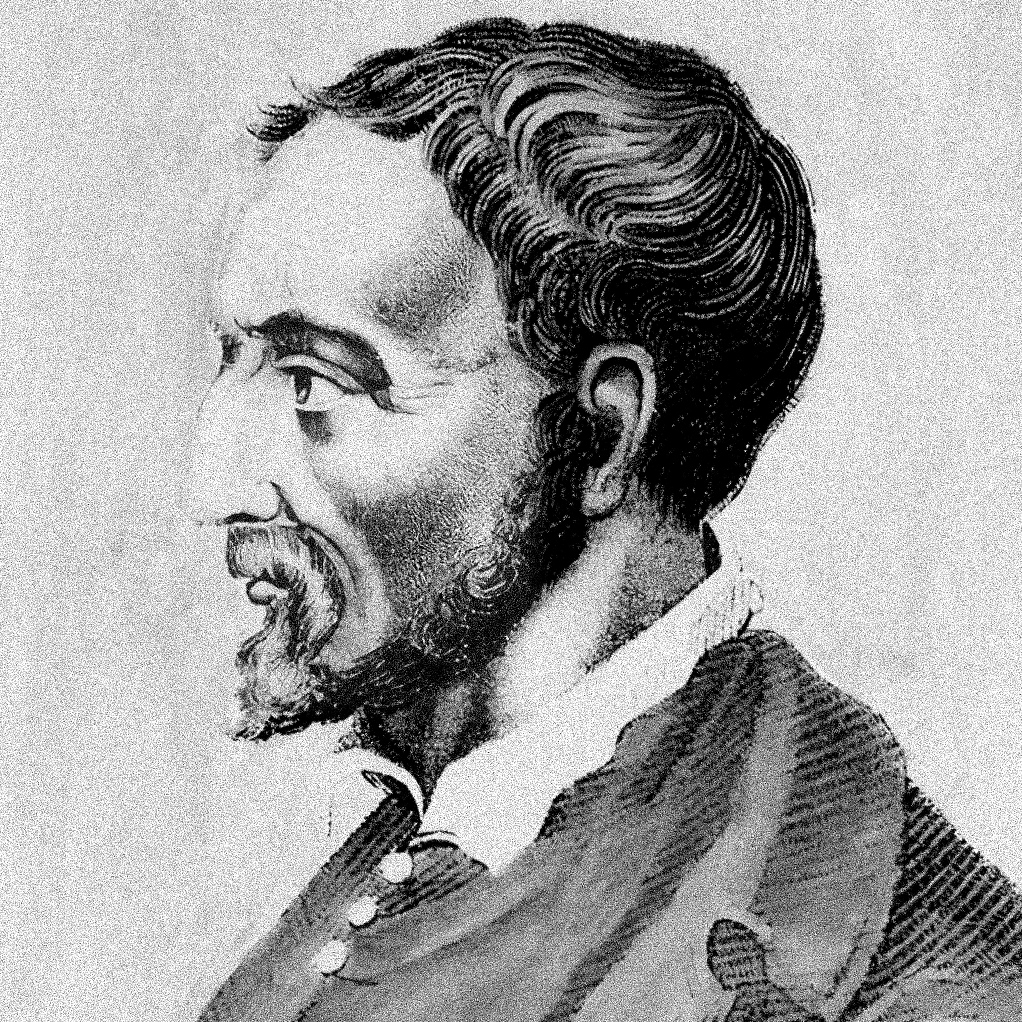
\includegraphics[width=\linewidth]{Images/ApendiceC/CARDANO.jpeg}
\textbf{Girolamo Cardano:} Nacido en Pavía en 1501, destacó por sus aportes significativos en la matemática; en áreas como la teoría de ecuaciones, la geometría y la probabilidad donde introdujó el número negativo en la teoría matemática y la resolución de ecuaciones de tercer grado. Además de sus aportes en matemáticas, Cardano comenzó a estudiar medicina a los 23 años, obteniendo su doctorado en 1525. Fue uno de los primeros médicos en practicar la autopsia y realizar estudios sobre la anatomía y fisiología humana. También, fue un astrólogo reconocido en su época y escribió varias obras sobre el tema. Falleció en Roma en 1576.
}

Los procesos que expondremos en esta apéndice, para obtener las fórmulas para resolver las ecuaciones de tercer y cuarto grados, se sustentan en los trabajos de los matemáticos italianos antes mencionados, y se basan en transformaciones especiales y complicadas de la ecuación respectiva, que bien pueden parecer artificiales y accidentales, pero que ocurrieron en la intensa búsqueda de métodos para resolver dichas ecuaciones.

\begin{observation}
    De la ecuación de primer grado, es decir
    $$ax+b=0$$
    solo diremos que su única solución es $\displaystyle x=-\frac{b}{a}$.
\end{observation}

\section{La definición del discriminante}

\begin{definition}\label{definicion:B.1.1}
    Consideremos la ecuación de grado $n \geq 2$ y coeficientes complejos dada por
    $$a_nx^n+\cdots +a_1x+a_0=0$$
    y sean $x_1, x_2, \dots, x_n$ sus raíces (no necesariamente distintas). Definimos el discriminante de esta ecuación como
    $$D=a_n^{2n-2}\prod_{1 \leq i < j \leq n}(x_i-x_j)^2.$$
\end{definition}

\begin{observation}
    En lugar de la ecuación
    $$a_nx^n+\cdots +a_1x+a_0=0$$
    de la definición anterior, podemos hablar del polinomio
    $$f(x)=a_nx^n+\cdots +a_1x+a_0.$$
    En este caso, se dice que
    $$D=a_n^{2n-2}\prod _{1 \leq i < j \leq n}(x_i-x_j)^2$$
    es el discriminante del polinomio $f(x)$.
\end{observation}

\section{Ecuación de segundo grado}

Consideremos la ecuación general de segundo grado, donde $a, b, c \in \CC$ y $a \neq 0$, con la incógnita $x$:
\begin{equation}
    ax^2+bx+c=0. \label{ecuaciongrado2}
\end{equation}
Si $r$ es raíz de \eqref{ecuaciongrado2}, entonces
\begin{equation}
    ar^2+br+c=0. \label{ecuaciongrado2.1}
\end{equation}
Multiplicando ambos miembros de \eqref{ecuaciongrado2.1} por $4a$, obtenemos
\begin{equation*}
    4a^2r^2+4abr+4ac=0. \label{ecuaciongrado2.2}
\end{equation*}
Sumando $b^2-4ac$ en ambos miembro de \eqref{ecuaciongrado2.2}, obtenemos
$$4a^2r^2+4abr+b^2=b^2-4ac $$
es decir,
$$(2ar+b)^2 = b^2-4ac$$
por tanto
$$2ar+b = \pm \sqrt{b^2-4ac}$$
y por ende,
$$r = \frac{-b \pm \sqrt{b^2-4ac}}{2a}$$\newpage
Nótese que $b^2-4ac$ es un número complejo, por lo que tiene dos raíces complejas $z$ y $w$, donde $w=-z$. Así que $\sqrt{b^2-4ac}$ representa a cualquiera, pero solo a una, de $z$ y $w$.

En resumen, las dos raíces (no necesariamente distintas) de la ecuación $ax^2+bx+c=0$ vienen dadas por la fórmula
$$x=\frac{-b \pm \sqrt{b^2-4ac}}{2a}.$$

\section{El discriminante de la ecuación de segundo grado}

Por la sección anterior, sabemos que las raíces de $ax^2+bx+c=0$ son
$$x_1=\frac{-b + \sqrt{b^2-4ac}}{2a} \hspace{0.5cm} \text{y} \hspace{0.5cm} x_2=\frac{-b - \sqrt{b^2-4ac}}{2a}.$$
Por lo que el discriminante de dicha ecuación es
$$D=a^2(x_1-x_2)^2,$$
es decir:
$$D=b^2-4ac.$$

\begin{observation}
    Si la ecuación de segundo grado $ax^2+bx+c=0$ es de coeficientes reales, entonces:
    \begin{enumerate}[label=\roman*.]
        \item Tiene dos raíces reales si y solo si $D>0$.
        \item Tiene una raíz real doble si y solo si $D=0$.
        \item Tienen dos raíces imaginarias diferentes si y solo si $D<0$.
    \end{enumerate}
\end{observation}

\section{La ecuación de tercer grado} \label{sec:B4}

Consideremos la ecuación general de tercer grado
\begin{equation}
    Ax^3+Bx^2+Cx+D=0 \label{ecuaciongrado3}
\end{equation}
con $A,  B,  C,  D \in \CC$ y $A \neq 0$ y con la incógnita $x$. Como $A \neq 0$, y puesto que la ecuación
$$\frac{1}{A} \left( Ax^3+Bx^2+Cx+D \right) =0$$
tiene las mismas raíces que la ecuación \eqref{ecuaciongrado3}, entonces no se pierde generalidad si en lugar de esta, escribimos
\begin{equation}
    x^3+bx^2+cx+d=0, \text{ con }  b,  c,  d \in \CC \label{ecuaciongrado3.1}
\end{equation}

Sustituyendo $\displaystyle x=y-\frac{b}{3}$ en \eqref{ecuaciongrado3.1}, se tiene que
$$\left( y-\frac{b}{3} \right)^3+b \left( y-\frac{b}{3} \right)^2+c \left( y-\frac{b}{3} \right) +d=0,$$
por tanto
$$y^3+\left( c-\frac{b^2}{3} \right) y + \left( d-\frac{bc}{3}+\frac{2b^3}{27} \right) =0.$$\newpage

En consecuencia, resolver la ecuación \eqref{ecuaciongrado3.1} se reduce a resolver la ecuación
$$y^3+py+q=0$$
donde
$$p=c-\frac{b^2}{3} \hspace{0.5cm} \text{y} \hspace{0.5cm} q=d-\frac{bc}{3}+\frac{2b^3}{27}.$$

Si $y_1$, $y_2$, $y_3$ son raíces de $y^3+py+q=0$, entonces:
$$x_1=y_1-\frac{b}{3} \hspace{1cm} x_2=y_2-\frac{b}{3} \hspace{1cm} x_3=y_3-\frac{b}{3}$$
son las raíces de \eqref{ecuaciongrado3.1}.

Resolveremos ahora la ecuación
\begin{equation}
    y^3+py+q=0. \label{ecuaciongrado3.2}
\end{equation}
Escribiendo $y=u+v$ en \eqref{ecuaciongrado3.2}, tenemos que
$$(u+v)^3+p(u+v)+q=0.$$
Desarrollando la expresión anterior, obtenemos
\begin{equation}
    u^3+v^3+q+(3uv+p)(u+v)=0. \label{ecuaciongrado3.3}
\end{equation}

Cualquiera que sea el valor numérico de la suma de $u$ y $v$, siempre podemos determinar a $u$ y $v$ imponiéndoles la condición adicional que su producto $uv$ sea un número prefijado. En efecto: supongamos que $u+v=r$ e impongamos la condición adicional $uv=s$, entonces $v=r-u$ y $uv=s$, por tanto $v=r-u$ y $u(r-u)=s$, por tanto $v=r-u$ y $u^2-r u+s=0$. En consecuencia $v=r-u$, y $u$ puede calcularse por la fórmula para resolver una ecuación de segundo grado. Esto demuestra lo que se afirmó.

Enseguida determinaremos a $u$ y $v$, sabiendo que la suma $u+v$ es raíz de la ecuación $y^3+p y+q=0$, e imponiendo la condición adicional
\begin{equation}
    uv=-\frac{p}{3}. \label{ecuaciongrado3.4}
\end{equation}
Sustituyendo \eqref{ecuaciongrado3.4} en \eqref{ecuaciongrado3.3}, tenemos que
\begin{equation}
    u^3+v^3+q=0. \label{ecuaciongrado3.5}
\end{equation}
De \eqref{ecuaciongrado3.4} y \eqref{ecuaciongrado3.5}, se sigue que
\begin{equation}
    u^3v^3=-\frac{p^3}{27} \label{ecuaciongrado3.6}
\end{equation}
y
\begin{equation}
    u^3+v^3=-q. \label{ecuaciongrado3.7}
\end{equation}

Puesto que
$$(z-u^3)(z-v^3)=z^2-(u^3+v^3)z+u^3v^3$$
entonces por \eqref{ecuaciongrado3.6} y \eqref{ecuaciongrado3.7}, $u^3$ y $v^3$ son las dos soluciones de la ecuación de segundo grado
\begin{equation}
    z^2+qz-\frac{p^3}{27}=0. \label{ecuaciongrado3.8}
\end{equation}

Por otro lado, las soluciones de la ecuación \eqref{ecuaciongrado3.8}, vienen dadas por
$$z_1=-\frac{q}{2}+\sqrt{\frac{q^2}{4}+\frac{p^3}{27}} \hspace{1cm} \text{y} \hspace{1cm} z_2=-\frac{q}{2}-\sqrt{\frac{q^2}{4}+\frac{p^3}{27}}.$$\newpage

Por tanto, podemos escribir
\begin{equation}
    u^3=z_1 \hspace{1cm} \text{y} \hspace{1cm} v^3=z_2. \label{ecuaciongrado3.9}
\end{equation}

Nótese que las anteriores ecuaciones son del tipo $x^n=z$, por lo que se pueden resolver mediante el método expuesto en el \hyperref[FUNDAMENTAL]{Apéndice C}. Cada una de dichas ecuaciones tiene tres raíces, digamos $u_1$, $u_2$, $u_3$, para $u^3=z_1$; y $v_1$, $v_2$, $v_3$, para $v^3=z_2$.

Resolviendo la ecuación $x^3=1$, tenemos que sus raíces son:
$$w^0=1 \hspace{1cm} w=\frac{-1+\sqrt{3}i}{2} \hspace{1cm} w^2=\frac{-1-\sqrt{3}i}{2}$$

Es fácil comprobar que las raíces de
$$u^3=z_1$$
son:
$$u_1 \hspace{1cm} u_2=wu_1 \hspace{1cm} u_3=w^2u_1;$$
y las raíces de
$$v^3=z_2$$
son:
$$v_1 \hspace{1cm} v_2=wv_1 \hspace{1cm} v_3=w^2v_1.$$

No perdamos de vista que estamos determinando valores de $u$ y $v$, de modo que la suma $u+v$ sea raíz de $y^3+py+q=0$, y que además $u$ y $v$ satisfagan la condición adicional $\displaystyle uv=-\frac{p}{3}$. Hemos determinado tres posibles valores $u_1,  u_2$ y $u_3$ para $u$; y tres posibles valores $v_1,  v_2$ y $v_3$ para $v$.

Pero observemos que
$$\left(u_i v_j\right)^3=-\frac{p^3}{27}$$
no implica que
$$u_i v_j=-\frac{p}{3},$$
para cada $i,  j=1,  2,  3$. Si elegimos $u_1$ y $v_1$ de modo que $\displaystyle u_1v_1=-\frac{p}{3}$, y a los que denotaremos por
\begin{equation}
    u_1=\sqrt[3]{\frac{-q}{2}+\sqrt{\frac{q^2}{4}+\frac{p^3}{27}}} \label{APPCOSIPA1}
\end{equation}
y
\begin{equation}
    v_1=\sqrt[3]{\frac{-q}{2}-\sqrt{\frac{q^2}{4}+\frac{p^3}{27}}}. \label{APPCOSIPA2}
\end{equation}

Entonces las raíces de
$$y^3+py+q=0$$
son
\begin{equation}
    y_1=u_1+v_1 \hspace{1cm} y_2=wu_1+w^2v_1 \hspace{1cm} y_3=w^2u_1+wv_1. \label{APPCOSIPA3}
\end{equation}
Las expresiones anteriores son conocidas como \textit{fórmulas de Cardano}, para calcular las raíces de la ecuación $y^3+py+q=0$.

\newpage
\section{El discriminante de la ecuación de tercer grado}\label{disc_tercergrado}

De acuerdo a las fórmulas de Cardano, y a la definición \ref{definicion:B.1.1}, el discriminante de la ecuación $y^3+py+q=0$ es
$$D=(y_1-y_2)^2(y_1-y_3)^2(y_2-y_3)^2.$$

Recordemos que
$$w=-\frac{1}{2}+\frac{1}{2}\sqrt{3}i$$
es raíz de la ecuación $x^3-1=0$, por tanto
$$w^3=1 \hspace{0.5cm} \text{y} \hspace{0.5cm} w^2+w+1=0$$
entonces
\begin{align*}
    y_1-y_2 &=(u_1+v_1)-\left(wu_1+w^2v_1\right) \\
    &=(1-w)u_1-w^2v_1+w^3v_1 \\
    &=(1-w)u_1+(1-w)\left(-w^2v_1\right) \\
    &=(1-w)\left(u_1-w^2v_1\right), \\
    & \\
    y_1-y_3 &=(u_1+v_1)-\left( w^2u_1+wv_1 \right) \\
    &=\left( 1-w^2 \right) u_1-wv_1+w^3v_1 \\
    &=\left( 1-w^2 \right) u_1+\left( 1-w^2 \right) (-wv_1) \\
    &=\left( 1-w^2 \right) (u_1-wv_1), \\
    & \\
    y_2-y_3 &=\left( wu_1+w^2v_1 \right) - \left( w^2u_1+wv_1 \right) \\
    &=\left( w-w^2 \right) u_1-wv_1+w^2v_1 \\
    &=\left( w-w^2 \right) u_1+\left( w-w^2 \right) (-v_1) \\
    &=\left( w-w^2 \right) (u_1-v_1).
\end{align*}

Además
\begin{align*}
    (1-w)\left( 1-w^2 \right) &= \left( \frac{3}{2}-\frac{\sqrt{3}}{2} i \right) \left( \frac{3}{2}+\frac{\sqrt{3}}{2} i \right) \\
    &=3
\end{align*}
y
$$w-w^2=\sqrt{3}i.$$
Puesto que
$$(x-1)(x-w)\left( x-w^2 \right) =x^3-1,$$
entonces
$$\left( \frac{u_1}{v_1} -1 \right) \left( \frac{u_1}{v_1} -w \right) \left( \frac{u_1}{v_1}-w^2 \right) = \left( \frac{u_1}{v_1} \right)^3 -1$$
por tanto
\begin{equation}
    (u_1-v_1)(u_1-wv_1)\left( u_1-w^2v_1 \right) = u^3_1-v^3_1 \label{onono}
\end{equation}
Por \eqref{ecuaciongrado3.9} de la sección \ref{sec:B4}, de \eqref{onono} se sigue que
$$(u_1-v_1)(u_1-wv_1)\left( u_1-w^2v_1 \right) = 2 \sqrt{\frac{q^2}{4}+\frac{p^3}{27}}.$$
En consecuencia,
\begin{align*}
    D &=\left[ (y_1-y_2)(y_1-y_3)(y_2-y_3) \right]^2 \\
    &=\left[ (1-w)\left( u_1-w^2v_1 \right) \left( 1-w^2 \right) (u_1-wv_1) \left( w-w^2 \right) (u_1-v_1) \right]^2 \\
    &=\left[ (1-w) \left( 1-w^2 \right) \left( w-w^2 \right) (u_1-v_1) (u_1-wv_1) \left( u_1-w^2v_1 \right) \right]^2 \\
    &=\left[ 3 \left( \sqrt{3}i \right) \left( 2 \sqrt{\frac{q^2}{4}+\frac{p^3}{27}} \right) \right]^2 \\
    &= -108 \left( \frac{q^2}{4} + \frac{p^3}{27} \right) \\
    &=-27q^2-4p^3
\end{align*}

En resumen, el discriminante de la ecuación
\begin{equation}
    y^3+py+q=0 \label{TOCOF}
\end{equation}
es
$$D=-4p^3-27q^2.$$
Si $y_1$, $y_2$, $y_3$ son las raíces de \eqref{TOCOF}, donde
$$p=c-\frac{b^2}{3}$$
y
$$q=d-\frac{bc}{3}+\frac{2b^3}{27}$$
se sabe que
$$x_1 = y_1-\frac{b}{3} \hspace{1cm} x_2 = y_2-\frac{b}{3} \hspace{1cm} x_3 = y_3-\frac{b}{3}$$
son las raíces de
$$x^3+bx^2+cx+d=0.$$
Por tanto
$$x_1-x_2=y_1-y_2 \hspace{1cm} x_1-x_3=y_1-y_3 \hspace{1cm} x_2-x_3=y_2-y_3.$$

En consecuencia, el discriminante de
$$x^3+bx^2+cx+d=0$$
es
$$\Delta =-4p^3-27q^2,$$
es decir,
\begin{align*}
    \Delta & = -4 \left( c - \frac{b^2}{3} \right)^3 - 27 \left( d - \frac{bc}{3} + \frac{2b^3}{27} \right)^2 \\
    & =18bcd-4b^3d+b^2c^2-4c^3-27d^2.
\end{align*}

\begin{observation}
    Consideremos el escenario en el cual la ecuación cúbica
    $$x^3+bx^2+cx+d=0$$
    posee coeficientes reales (y por consiguiente, también su ecuación asociada $y^3 + py + q=0$ tiene coeficientes reales). Dado que esta ecuación es de grado impar, garantiza la existencia de al menos una raíz real. Por lo tanto, se presentan las siguientes tres posibilidades en relación con sus raíces:\newpage
    \begin{enumerate}[label=\roman*.]
        \item Si $\Delta >0$, entonces tiene una raíz real y dos raíces complejas conjugadas.
        \item Si $\Delta =0$, entonces tiene tres raíces reales y por lo menos dos de ellas son iguales.
        \item Si $\Delta <0$, entonces tiene tres raíces reales diferentes.
    \end{enumerate}
\end{observation}

\begin{example}
    Resuelva la ecuación
    $$y^3+3y^2-3y-14=0.$$
    \solucion Usando la sustitución $y=x-1$ reducimos esta ecuación a la forma
    $$x^3-6x-9=0.$$
    Notemos que $p=-6$ y $q=-9$, por lo cual
    $$\frac{q^2}{4}+\frac{p^3}{27}=\frac{49}{4}>0.$$
    Entonces, la ecuación
    $$x^3-6x-9=0$$
    tiene una raíz real y dos raíces complejas conjugadas. Según las expresiones \eqref{APPCOSIPA1} y \eqref{APPCOSIPA2},
    $$u_1=\sqrt[3]{\frac{9}{2}+\frac{7}{2}}=\sqrt[3]{8} \quad \text{ y } \quad v_1=\sqrt[3]{\frac{9}{2}-\frac{7}{2}}=\sqrt[3]{1}.$$
    Por consiguiente, $u_1=2$ y $v_1=1$, es decir, $x_1=3$. Las otras dos raíces se hallan por las fórmulas \eqref{APPCOSIPA3}:
    $$x_2 = - \frac{3}{2} + \frac{\sqrt{3}}{2}i \quad \text{ y } \quad x_2 = - \frac{3}{2} - \frac{\sqrt{3}}{2}.$$
    De aquí se deduce que las raíces de la ecuación dada son:
    $$y_1 = 2, \quad y_2 = - \frac{5}{2} + \frac{\sqrt{3}}{2}i, \quad y_3 = - \frac{5}{2} - \frac{\sqrt{3}}{2}i.$$
\end{example}

\begin{example}
    Resuelva la ecuación
    $$x^3-12x+16=0.$$
    \solucion Notemos que $p=-12$ y $q=16$, por lo tanto
    $$\frac{q^2}{4}+\frac{p^3}{27}=0.$$
    De esta ecuación, obtenemos $u_1=\sqrt[3]{-8}$, lo que implica que $u_1=-2$. En consecuencia, las raíces son $x_1=-4$ y $x_2=2=x_3$.
\end{example}

\begin{example}
    Resuelva la ecuación
    $$x^3 - 9x^2 + 36x - 80 = 0.$$
    \solucion Usando la sustitución $x = y + 3$ reducimos esta ecuación a la forma
    $$y^3 + 9y - 26 = 0.$$
    Notemos que $p=9$ y $q=-26$, por lo cual
    $$\frac{q^2}{4}+\frac{p^3}{27}=196>0.$$
    Entonces, la ecuación
    $$y^3 + 9y - 26 = 0$$
    tiene una raíz real y dos raíces complejas conjugadas. Según las expresiones \eqref{APPCOSIPA1} y \eqref{APPCOSIPA2},
    $$u_1=\sqrt[3]{13 + \sqrt{196}}=\sqrt[3]{27} \quad \text{ y } \quad v_1=\sqrt[3]{13 - \sqrt{196}}=\sqrt[3]{-1}.$$
    Por consiguiente, $u_1=3$ y $v_1=-1$, es decir, $y_1=2$. Las otras dos raíces se hallan por las fórmulas \eqref{APPCOSIPA3}:
    $$y_2=-1+2\sqrt{3}i, \quad y_3=-1-2\sqrt{3}i.$$
    De aquí se deduce que las raíces de la ecuación dada son:
    $$x_1=5, \quad x_2=2+2\sqrt{3}i, \quad x_3=2-2\sqrt{3}i.$$
\end{example}

\section{La ecuación de cuarto grado}

Consideremos la ecuación general de cuarto grado,
\begin{equation}
    Ax^4+Bx^3+Cx^2+Dx+E=0, \label{ecuacioncuarto7.1}
\end{equation}
donde $A,  B,  C,  D,  E \in \CC$ y $A \neq 0$, con la incógnita $x$.

Como $A \neq 0$, y puesto que la ecuación
$$\frac{1}{A} \left( Ax^4+Bx^3+Cx^2+Dx+E \right) =0$$
tiene las mismas raíces que la ecuación \eqref{ecuacioncuarto7.1}, entonces no se pierde generalidad si en lugar de esta, escribimos
\begin{equation}
    x^4+ax^3+bx^2+cx+d=0 \label{ecuacioncuarto7.2}
\end{equation}

Si la ecuación \eqref{ecuacioncuarto7.2} la escribimos en la forma
$$x^4+ax^3=-bx^2-cx-d$$
y sumamos $\displaystyle \frac{a^2}{4}x^2$ a ambos miembros de la ecuación, entonces
$$x^4+ax^3+\frac{a^2}{4}x^2=\frac{a^2}{4}x^2-bx^2-cx-d,$$
donde se sigue que
\begin{equation}
    \left( x^2+\frac{a}{2}x \right)^2 = \left( \frac{a^2}{4}-b \right) x^2-cx-d. \label{ecuacioncuarto7.3}
\end{equation}

Si el miembro derecho de la ecuación \eqref{ecuacioncuarto7.3} fuera un cuadrado perfecto, es decir, si fuera de la forma $(ex+f)^2$, entonces resolver dicha expresión y resolver \eqref{ecuacioncuarto7.2} sería inmediato. Pero en general dicho miembro derecho no es un cuadrado perfecto.

Sumando
$$\left( x^2+\frac{a}{2}x \right) y + \frac{y^2}{4}$$
a ambos miembros de \eqref{ecuacioncuarto7.3}, tenemos que
$$\left( x^2+\frac{a}{2}x \right)^2 + \left( x^2+\frac{a}{2}x \right) y + \frac{y^2}{4} = \left( \frac{a^2}{4}-b \right) x^2-cx-d + \left( x^2+\frac{a}{2}x \right) y + \frac{y^2}{4},$$
por tanto
\begin{equation}
    \left( x^2+\frac{a}{2}x+\frac{y}{2} \right)^2 = \left( \frac{a^2}{4}-b+y \right) x^2 + \left( -c+\frac{1}{2} ay \right) x+ \left( -d + \frac{1}{4} y^2 \right). \label{ecuacioncuarto7.4}
\end{equation}

Vamos a determinar $y$ de modo que el miembro derecho de la expresión \eqref{ecuacioncuarto7.4} sea un cuadrado perfecto. Para esto observemos que
$$Ax^2+Bx+C=(ex+f)^2,$$
si y solo si
$$B^2-4AC=0.$$
En efecto
\begin{align*}
    Ax^2+Bx+C=(ex+f)^2 & \Longrightarrow Ax^2+Bx+C=e^2x^2+2efx+f^2 \\ 
    & \Longrightarrow A=e^2, \; B=2ef, \; C=f^2 \\ 
    & \Longrightarrow B^2-4AC=0.
\end{align*}
Recíprocamente, si $B^2-4AC=0$, entonces
\begin{align*}
    Ax^2+Bx+C &=A \left( x^2+\frac{B}{A}x+\frac{C}{A} \right) \\
    &=A \left( x+\frac{B}{2A}-\frac{\sqrt{B^2-4AC}}{2A} \right) \left( x+\frac{B}{2A}+\frac{\sqrt{B^2-4AC}}{2A} \right) \\
    &=A \left( x+\frac{B}{2A} \right)^2 \\
    &=\left( \sqrt{A}x+\frac{B}{2\sqrt{A}} \right)^2 \\
    &=(ex+f)^2
\end{align*}
con $e=\sqrt{A}$ y $\displaystyle f=\frac{B}{2\sqrt{A}}$. En consecuencia, el miembro derecho de \eqref{ecuacioncuarto7.4} será un cuadrado perfecto, es decir,
$$\left( \frac{a^2}{4}-b+y \right) x^2+\left( -c+\frac{1}{2}ay \right) x + \left( -d+\frac{1}{4}y^2 \right) = (ex+f)^2,$$
si y solo si
$$\left( -c+\frac{1}{2}ay \right)^2 -4 \left( \frac{a^2}{4}-b+y \right) \left( -d+\frac{1}{4}y^2 \right) =0,$$
si y solo si
$$c^2-acy+\frac{1}{4}a^2y^2-4 \left( -\frac{a^2d}{4}+\frac{a^2y^2}{16}+bd-\frac{1}{4}by^2-dy+\frac{1}{4} y^3 \right) =0,$$
si y solo si
$$-y^3+by^2+(4d-ac)y+a^2d-4bd+c^2=0,$$
si y solo si
\begin{equation}
    y^3-by^2+(ac-4d)y+\left(4bd-a^2d-c^2\right)=0. \label{ecuacioncuarto7.5}
\end{equation}

Si $y_0$ es una solución cualquiera de la ecuación cúbica \eqref{ecuacioncuarto7.5}, la cual es llamada la \textit{resolvente} de la ecuación \eqref{ecuacioncuarto7.2} de grado cuatro, entonces por \eqref{ecuacioncuarto7.4} tenemos que:
$$\left( x^2+\frac{a}{2}x+\frac{y_0}{2} \right)^2 = (ex+f)^2$$\newpage\noindent
por tanto
\begin{equation}
    x^2+\frac{a}{2}x+\frac{y_0}{2}=ex+f \label{ecuacioncuarto7.6}
\end{equation}
y
\begin{equation}
    x^2+\frac{a}{2}x+\frac{y_0}{2}=-ex-f. \label{ecuacioncuarto7.7}
\end{equation}

Las cuatro soluciones de \eqref{ecuacioncuarto7.6} y \eqref{ecuacioncuarto7.7} son las raíces de \eqref{ecuacioncuarto7.2}.

\section{La ecuación de quinto grado}\label{ecuacion_quinto_grado}

Las fórmulas para la resolución de las ecuaciones de tercero y cuarto grado fueron descubiertas ya en el siglo XVI. Al mismo tiempo comenzaron las búsquedas de fórmulas para la resolución de las ecuaciones de quinto grado y de grados superiores. Señalemos que la forma general de una ecuación de $n$-ésimo grado es:
$$a_nx^n+a_{n-1}x^{n-1}+\cdots +a_1 x+a_0 = 0$$
Estas búsquedas continuaron sin éxito hasta comienzos del siglo XIX, cuando por fin fue demostrado el siguiente resultado extraordinario:
\begin{tcolorbox}[
        theorem style=change break,
        enhanced,
        breakable,
        boxrule=0pt,
        frame hidden,
        borderline west={3pt}{0pt}{black},
        colback=gray!20,
        coltitle=gray!90,
        attach title to upper={\ },
        sharp corners,
        fonttitle=\bfseries,
        fontupper=\normalsize
    ]
    Para ningún $n$, mayor o igual a cinco puede hallarse formula que exprese las raíces de cualquiera ecuación de $n$-ésimo grado mediante sus coeficientes por radicales.
\end{tcolorbox}

Más aún, para cualquier $n$ mayor o igual a cinco se puede indicar una ecuación de $n$-ésimo grado con coeficientes enteros, cuyas raíces no pueden expresarse mediante radicales. Tal es, por ejemplo, la ecuación
$$x^5 - 4x - 2 = 0.$$
Puede demostrarse que esta ecuación tiene cinco raíces, tres reales y dos complejas, pero ninguna de ellas puede expresarse mediante radicales, es decir, esta ecuación es “irresoluble por radicales”. De este modo la reserva de números, reales o complejos que son raíces de las ecuaciones con coeficientes enteros (estos números se denominan algebraicos en contraposición a los números trascendentes que no son raíces de ninguna ecuación con coeficientes enteros), es mucho más amplia que la reserva de números que se expresan por radicales.

La inexistencia de fórmulas generales para la resolución por radicales de las ecuaciones de $n$-ésimo grado cuando $n \geq 5$ fue demostrada por Abel (1802-1829). La existencia de ecuaciones con coeficientes enteros irresolubles por radicales fue establecida por Galois (1811-1832), quien también halló las condiciones en las cuales la ecuación puede resolverse por radicales. Todos estos resultados exigieron la creación de una nueva y profunda teoría, la teoría de grupos. El concepto de grupo permitió agotar la cuestión referente a la resolución de ecuaciones por radicales, habiendo hallado más tarde numerosas aplicaciones en diferentes ramas de la matemática y fuera de sus límites, convirtiéndose en uno de los objetos más importantes de estudio en el álgebra.

El hecho de que no existen fórmulas para resolver las ecuaciones de $n$-ésimo grado cuando $n \geq 5$ no provoca dificultades serias en lo que respecta a la búsqueda práctica de las raíces de las ecuaciones. Esto se compensa totalmente por los numerosos métodos de resolución aproximada de las ecuaciones, que incluso en el caso de las ecuaciones cúbicas conducen al objetivo con mayor rapidez que utilizando la fórmula y extrayendo, a continuación, en forma aproximada los radicales reales. No obstante, la existencia de fórmulas para las ecuaciones de segundo, tercero y cuarto grados permitió demostrar que estas ecuaciones poseen respectivamente dos, tres o cuatro raíces.

En este apéndice, nos hemos referido aquí solamente a las ecuaciones de un cierto grado con una incógnita. El origen de esta teoría se remonta al álgebra elemental, en la que luego del estudio de ecuaciones de primer grado, se pasan al estudio de ecuaciones cuadráticas. Pero en el álgebra elemental también se dio un paso en otra dirección: luego de estudiar una ecuación de primer grado con una incógnita se pasó a considerar el sistema de dos ecuaciones de primer grado con dos incógnitas y el sistema de tres ecuaciones con tres incógnitas. El desarrollo de esta teoría se da en el curso de Álgebra II dado en la ESFM. En el mismo se estudian los métodos de resolución de cualesquiera sistemas de $n$ ecuaciones de primer grado con $n$ incógnitas, así como también los métodos para hallar la solución de aquellos sistemas de ecuaciones de primer grado en los cuales el número de ecuaciones no es igual al número de incógnitas. La teoría de los sistemas de ecuaciones de primer grado, así como otras, que le son afines, en particular, la teoría de matrices, forman una rama especial del álgebra, el álgebra lineal; de entre todas las partes del álgebra, ésta es la principal debido a sus aplicaciones en geometría y otras ramas de las matemáticas, así como también en física y mecánica teórica.

Por otra parte, tanto la teoría de las ecuaciones algebraicas como el álgebra lineal, en gran medida, pueden ser considerados actualmente como partes acabadas de la ciencia. Las necesidades de ramas contiguas de la matemática y la física condujeron a que en el álgebra pasó a primer plano el estudio de los conjuntos en los cuales están dadas las operaciones algebraicas. Además de la teoría de los campos, dentro de la cual entran la teoría de los números algebraicos y la teoría de las funciones algebraicas, ahora también se desarrolla la teoría de los anillos.